\documentclass[12pt]{article}
\usepackage{graphicx}
\usepackage{amsmath}
\usepackage{mathtools}
\usepackage{gensymb}

\newcommand{\mydet}[1]{\ensuremath{\begin{vmatrix}#1\end{vmatrix}}}
\providecommand{\brak}[1]{\ensuremath{\left(#1\right)}}
\providecommand{\norm}[1]{\left\lVert#1\right\rVert}
\newcommand{\solution}{\noindent \textbf{Solution: }}
\newcommand{\myvec}[1]{\ensuremath{\begin{pmatrix}#1\end{pmatrix}}}
\let\vec\mathbf

\begin{document}
\begin{center}
\textbf\large{CHAPTER-7 \\ COORDINATE GEOMETRY}
\end{center}
\section*{Excercise 7.4}

Q2. Find a relation between x and y if the points $\vec(x, y), \vec(1, 2) \text{ and } \vec(7, 0)$ are collinear.
\\
\solution
\\
The coordinates are given as
	\begin{align}
	\vec{A} = \myvec{
		x\\
		y\\
		},
	\vec{B} = \myvec{
		1\\
		2\\
		},
	\vec{C} = \myvec{
		7\\
		0\\
		}
	\end{align}
	\begin{align}
\vec{D} &=\brak{\vec{A}-\vec{B}} = \brak{\myvec{x \\y } - \myvec{1 \\2 } } = \myvec{x-1 \\ y-2 }\\
\vec{E} &= \brak{\vec{A}-\vec{C}} = \brak{\myvec{x \\ y } - \myvec{7 \\0} } = \myvec{x-7 \\y}
\end{align}
 If points on a line  are  collinear, rank of matrix is " 1 "then the vectors are in linearly dependent.
For $2\times2$ matrix Rank = 1 means Determinant is 0.
Through pivoting,we obtain
\begin{align}
	\vec{F} &={\myvec{\vec{D}^{\top}\\ \vec{E}^{\top}}}
\end{align}
\begin{align}
\begin{split}
\myvec{
x-1 & y-2
 \\
x-7 & y 
}
\end{split}
\end{align}

\begin{align}
\label{eq:chem_balance_mat_row}
\myvec{
x-1 & y-2
\\
x-7 & y
}
\xleftrightarrow[]{R_2 = R_2-R_1}
\myvec{
  x-1 & y-2
  \\
	  -6 & 2                 
	  }
	  \\
	\xleftrightarrow[]{R_2 = \frac{R_2}{-6}(x-1)-R_1}
\myvec{
x-1 & y-2
\\
	0 & -\frac{1}{3}(x-1)-(y-2)
}
\end{align}
If the rank of the matrix has to be 1 , then:
\begin{align}
		-\frac{1}{3}(x-1)-(y-2)=0\\
	 	\vec{x+3y-7=0}
\end{align}
Suppose, if $x=-2,y=3$ , then rank of F is equal to one which is collinear as shown in Figure:\ref    {fig:Fig}
\begin{figure}[!h]
	\begin{center} 
	    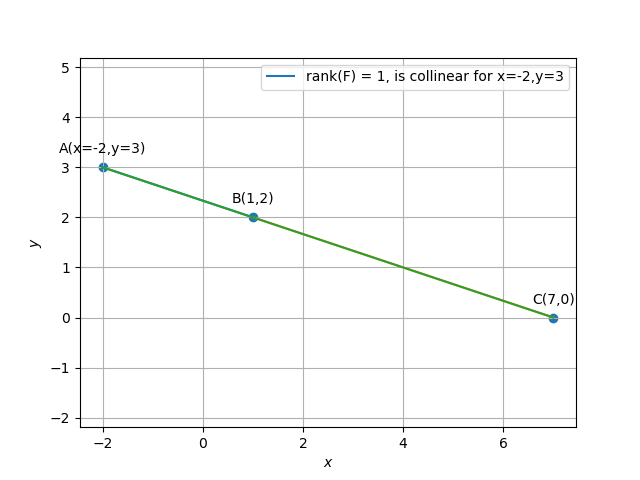
\includegraphics[width=\columnwidth]{./figs/sc1.png}
	\end{center}
\caption{}
\label{fig:Fig}
\end{figure}
\end{document}
